% !TeX root = ../complete.tex
\section{\lr{Logical Effort} مسیر و اندازه‌گذاری گیت‌ها}
\label{sec:delay-path-model}

در \hyperref[sec:delay-linear-model]{مدل خطی تأخیر تک‌گیت} دیدیم
که افزایش اندازه گیت، راه‌اندازی بار خروجی را آسان‌تر می‌کند.
در مسیر چندمرحله‌ای، ورودی همان گیت بخشی از بار مرحله پیشین است.
بنابراین انتخاب اندازه باید با درنظرگرفتن تأخیر مجموع مراحل انجام
شود. ابتدا یک مسیر مشخص را اندازه‌گذاری می‌کنیم و سپس مسیرهایی
با تعداد مراحل متفاوت را مقایسه می‌کنیم
\cite[بخش \secnum{۴.۵}، صفحات ۱۶۳ تا ۱۷۳]{weste}
\cite[اسلایدهای ۱۳ تا ۲۷]{logicaleffortslides}.

\subsection{بار مسیر و اثر انشعاب}
\label{sec:delay-path-branching}

از یک ورودی تا یک خروجی مشخص، \(N\) گیت روی مسیر را به‌ترتیب
شماره‌گذاری می‌کنیم. \(C_i\) ظرفیت همان ورودی از گیت \(i\)
است که مسیر از آن عبور می‌کند. برای یکسان‌بودن نمادگذاری،
\(C_{N+1}\) بار انتهاییِ روی مسیر است. بارهای موازی خارج از
مسیر در خروجی مرحله \(i\) را با \(C_{\mathrm{off},i}\)
نشان می‌دهیم. نسبت بار کل به بار روی مسیر، \lr{Branching Effort}
مرحله است. با این قرارداد، رابطه بار و \lr{Electrical Effort}
به‌صورت زیر نوشته می‌شود
\cite[روابط \secnum{۴.۳۵} تا \secnum{۴.۳۷}، صفحه ۱۶۴]{weste}
\cite[اسلایدهای ۱۳ تا ۱۶]{logicaleffortslides}.
\begin{equation}
  b_i=\frac{C_{i+1}+C_{\mathrm{off},i}}{C_{i+1}},
  \qquad
  h_i=\frac{C_{i+1}+C_{\mathrm{off},i}}{C_i}
     =b_i\frac{C_{i+1}}{C_i}.
  \label{eq:delay-path-branching}
\end{equation}
بدون بار جانبی، \(b_i=1\) است. اگر خروجی یک گیت دو ورودی
هم‌اندازه را راه‌اندازی کند و مسیر از یکی از آن‌ها بگذرد،
بار کل دو برابر بار روی مسیر و \(b_i=2\) است.

\(G\) حاصل‌ضرب \lr{Logical Effort} گیت‌های مسیر،
\(B\) حاصل‌ضرب ضرایب انشعاب و \(H\) نسبت ظرفیت انتهایی
به ظرفیت ورودی مسیر است. با ضرب \(h_i\)ها، ظرفیت هر گیت
میانی یک‌بار در صورت و یک‌بار در مخرج ظاهر می‌شود. در نتیجه،
حاصل‌ضرب آن‌ها \(B(C_{N+1}/C_1)\) است. با استفاده از
\(f_i=g_i h_i\) در رابطه \eqref{eq:delay-normalized-gate}،
\lr{Path Effort} با نماد \(F\) چنین به دست می‌آید
\cite[روابط \secnum{۴.۳۲} تا \secnum{۴.۳۷}، صفحه ۱۶۴]{weste}.
\begin{equation}
  G=\prod_{i=1}^{N}g_i,\qquad
  B=\prod_{i=1}^{N}b_i,\qquad
  H=\frac{C_{N+1}}{C_1},\qquad
  F=\prod_{i=1}^{N}f_i=GBH.
  \label{eq:delay-path-effort}
\end{equation}
همه این نسبت‌ها بی‌بعدند. نرخ انشعاب در هر گره از ظرفیت
ورودی شاخه‌ها تعیین می‌شود. در دو شاخه با بار متفاوت،
شمردن تعداد شاخه‌ها برای محاسبه \(b_i\) کافی نیست.

\subsection{کمینه تأخیر برای مسیر مشخص}
\label{sec:delay-path-equal-effort}

نوع گیت‌ها و تعداد مراحل را ثابت بگیرید. همچنین فرض کنید
ظرفیت ابتدا و بار انتهای مسیر معلوم‌اند، \(b_i\)ها با
اندازه‌گذاری ثابت می‌مانند و \(p_i\)ها را در تقریب خطی ثابت
می‌گیریم. ثابت‌ماندن \(b_i\) در یک انشعاب هم‌اندازه وقتی
برقرار است که اندازه ورودی شاخه‌های آن انشعاب با هم تغییر کند.
تأخیر نرمال‌شده مسیر \(D\)، مجموع تأخیر گیت‌هاست. اگر
\(P\) مجموع تأخیرهای \lr{Parasitic} باشد، تنها سهمی که در
این مدل با تغییر اندازه بهینه می‌شود، مجموع \(f_i\)هاست
\cite[روابط \secnum{۴.۳۸} تا \secnum{۴.۴۰}، صفحات ۱۶۴ و ۱۶۵]{weste}
\cite[اسلایدهای ۱۷ و ۱۸]{logicaleffortslides}.
\begin{equation}
  D=\sum_{i=1}^{N}d_i=\sum_{i=1}^{N}f_i+P,
  \qquad P=\sum_{i=1}^{N}p_i.
  \label{eq:delay-path-sum}
\end{equation}
برای دو مقدار مثبت \(a\) و \(b\) با حاصل‌ضرب ثابت، جایگزینی
هر دو با \(\sqrt{ab}\) مجموع را کاهش می‌دهد، زیرا
\(a+b-2\sqrt{ab}=(\sqrt a-\sqrt b)^2\) نامنفی است.
صورت کلی این مقایسه برای \(N\) مقدار مثبت می‌گوید میانگین
حسابی، یعنی مجموع تقسیم بر \(N\)، دست‌کم به اندازه میانگین
هندسی است. میانگین هندسی ریشه مرتبه \(N\) از حاصل‌ضرب است.
نماد \(F^{1/N}\) عدد مثبتی است که توان \(N\)ام آن \(F\)
می‌شود. در اینجا \(F\) ثابت است و برابری دو میانگین زمانی
رخ می‌دهد که همه \(f_i\)ها برابر باشند. پس مقدار مشترک
\(\widehat f\) و کمینه تأخیر برای مسیر ثابت چنین‌اند.
\begin{equation}
  \widehat f=F^{1/N},
  \qquad
  D_{\min}(N)=N F^{1/N}+P.
  \label{eq:delay-path-minimum}
\end{equation}
برابری \(f_i\)ها به معنی برابری \(d_i\)ها نیست. اگر
پارامترهای \(p_i\) متفاوت باشند، تأخیر کل مراحل نیز متفاوت است.

برای رسیدن به این کمینه در مدل پیوسته، از بار معلوم انتهای
مسیر آغاز می‌کنیم. با قرار دادن \(f_i=\widehat f\) در رابطه
\eqref{eq:delay-path-branching} و حل برای \(C_i\)، داریم
\cite[رابطه \secnum{۴.۴۱}، صفحه ۱۶۵]{weste}
\cite[اسلاید ۲۰]{logicaleffortslides}.
\begin{equation}
  C_i=
  \frac{g_i\bigl(C_{i+1}+C_{\mathrm{off},i}\bigr)}{\widehat f}
  =\frac{g_i b_i C_{i+1}}{\widehat f}.
  \label{eq:delay-path-backward-sizing}
\end{equation}
با تکرار از خروجی به ورودی، اندازه‌ها به دست می‌آیند. مقدار
محاسبه‌شده \(C_1\) باید با ظرفیت ورودی مجاز مطابقت داشته باشد.
اگر اندازه‌های قابل‌انتخاب کتابخانه گسسته‌اند، تأخیر را پس از
انتخاب اندازه‌های واقعی دوباره محاسبه می‌کنیم.

\subsection{مثال مسیر سه‌مرحله‌ای}
\label{sec:delay-three-stage-path}

در شکل \ref{fig:delay-three-stage-path}، مسیر از \(A\) تا \(B\)
از \lr{NAND2}، \lr{NAND3} و \lr{NOR2} می‌گذرد.
\(C\) واحد ظرفیت ورودی ترانزیستور است. ورودی مرحله اول
\(8C\) و بار نهایی \(45C\) است. \(xC\) ظرفیت هر ورودی
نشان‌داده‌شده از یک \lr{NAND3} و \(yC\) ظرفیت ورودی
نشان‌داده‌شده از یک \lr{NOR2} است. شاخه‌های منشعب از هر
خروجی، ورودی‌هایی با ظرفیت برابر دارند
\cite[مثال \secnum{۴.۱۳}، شکل‌های \secnum{۴.۳۱} و
\secnum{۴.۳۲}، صفحات ۱۶۵ و ۱۶۶]{weste}
\cite[اسلایدهای ۲۱ تا ۲۳]{logicaleffortslides}.

\begin{figure}[htbp]
  \centering
  \begin{latin}
  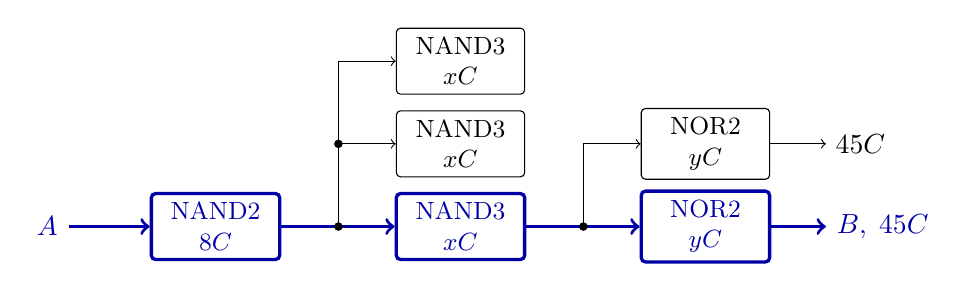
\begin{tikzpicture}[x=1.02cm,y=1cm,
      gate/.style={draw,rounded corners=1.5pt,minimum width=1.63cm,
        minimum height=0.75cm,align=center,font=\small},
      active/.style={very thick,blue!65!black}]
    \node[gate,active] (first) at (1.95,0) {NAND2\\\(8C\)};
    \node[gate,active] (middle) at (5.0,0) {NAND3\\\(xC\)};
    \node[gate] (upperMiddle) at (5.0,1.05) {NAND3\\\(xC\)};
    \node[gate] (topMiddle) at (5.0,2.1) {NAND3\\\(xC\)};
    \node[gate,active] (last) at (8.05,0) {NOR2\\\(yC\)};
    \node[gate] (upperLast) at (8.05,1.05) {NOR2\\\(yC\)};
    \draw[active,->] (0.12,0) node[left] {\(A\)} -- (first.west);
    \draw[active,->] (first.east) -- (middle.west);
    \draw[active,->] (middle.east) -- (last.west);
    \draw[active,->] (last.east) -- (9.55,0) node[right] {\(B,\;45C\)};
    \draw[->] (3.48,0) |- (upperMiddle.west);
    \draw[->] (3.48,1.05) |- (topMiddle.west);
    \draw[->] (6.53,0) |- (upperLast.west);
    \draw[->] (upperLast.east) -- (9.55,1.05) node[right] {\(45C\)};
    \fill (3.48,0) circle (1.55pt);
    \fill (3.48,1.05) circle (1.55pt);
    \fill (6.53,0) circle (1.55pt);
  \end{tikzpicture}
  \end{latin}
  \caption{مسیر سه‌مرحله‌ای از \(A\) تا \(B\) با خط پررنگ.
  ظرفیت ورودی‌های مربوط با \(8C\)، \(xC\) و \(yC\) و بار
  انتهایی با \(45C\) مشخص شده‌اند. شکل از روی اتصال‌های اسلاید
  ۲۱ \cite{logicaleffortslides} بازترسیم شده است.}
  \label{fig:delay-three-stage-path}
\end{figure}

بار خروجی مرحله اول \(3xC\)، بار خروجی مرحله دوم \(2yC\)
و بار خروجی مرحله سوم \(45C\) است. پس \(B=3\cdot2=6\).
با ضرایب جدول \ref{tab:delay-simple-gates} و با فرض
\(p_{\mathrm{inv}}=1\)، حاصل‌ضرب‌ها و جمع تأخیر بی‌بار چنین‌اند.
\[
  G=\frac43\cdot\frac53\cdot\frac53=\frac{100}{27},
  \qquad H=\frac{45}{8},\qquad F=125,\qquad P=2+3+2=7.
\]
ریشه سوم ۱۲۵ برابر ۵ است. بنابراین از رابطه
\eqref{eq:delay-path-minimum}، تأخیر مسیر \(3\cdot5+7=22\)
به دست می‌آید. اگر \(\tau=\qty{3}{\pico\second}\) باشد،
تأخیر \(\qty{66}{\pico\second}\) است. با مدل
\hyperref[sec:delay-fo4]{\lr{FO4}} این مقدار معادل
\num{4.4} برابر تأخیر مرجع \lr{FO4} است.

برای اندازه‌گذاری، ابتدا ظرفیت ورودی \lr{NOR2} را از بار معلوم
خروجی و سپس ظرفیت ورودی \lr{NAND3} را از بار هر دو
\lr{NOR2} حساب می‌کنیم. در پایان، رابطه
\eqref{eq:delay-path-backward-sizing} ظرفیت ورودی مرحله اول
را نیز بازتولید می‌کند.
\[
  y=\frac{(5/3)\cdot45}{5}=15,\qquad
  x=\frac{(5/3)\cdot(2y)}{5}=10,\qquad
  \frac{(4/3)\cdot(3x)}{5}=8.
\]
در این مدل، ظرفیت هر ورودی با مجموع عرض نسبی \lr{nMOS} و
\lr{pMOS} همان ورودی متناسب است. در \lr{NOR2}، نسبت
عرض \lr{pMOS} به \lr{nMOS} برابر ۴ به ۱ است. برای مجموع ۱۵،
عرض نسبی \lr{pMOS} برابر ۱۲ و عرض \lr{nMOS} برابر ۳ می‌شود.
برای \lr{NAND3}، تقسیم مجموع ۱۰ به نسبت ۳ به ۲، به‌ترتیب
عرض‌های ۶ و ۴ را برای \lr{nMOS} و \lr{pMOS} می‌دهد.
برای کنترل نهایی، با بارهای \(30C\)، \(30C\) و \(45C\)،
هر سه \(f_i\) برابر ۵ و تأخیرهای \(d_i\) به‌ترتیب ۷،
۸ و ۷ هستند.

\subsection{انتخاب تعداد مراحل}
\label{sec:delay-path-stage-count}

در یک مسیر با \(N_0\) مرحله و مجموع \(P_0\)، افزودن
\lr{Inverter} در انتهای مسیر می‌تواند بار بزرگ را میان مراحل
توزیع کند. در مدل کتاب فرض می‌شود \(F\) ثابت می‌ماند، زیرا
گیت اضافه \(g=1\) دارد و \(H\) و \(B\) ثابت فرض می‌شوند.
اگر در یک گره، بار روی مسیر از \(4C\) به \(2C\) برسد و
بار خارج از مسیر \(4C\) بماند، ضریب انشعاب آن گره از
\((4C+4C)/(4C)=2\) به \((2C+4C)/(2C)=3\) می‌رسد.
با تغییر \(B\)، مقدار \(F=GBH\) را برای هر گزینه دوباره
محاسبه می‌کنیم. در حالت \(F\) ثابت، هر مرحله اضافه \(p_{\mathrm{inv}}\)
به تأخیر بی‌بار می‌افزاید. بنابراین برای \(N\ge N_0\)، تأخیر
کمینه با تعداد مراحل \(N\) چنین است
\cite[روابط \secnum{۴.۴۲} و \secnum{۴.۴۳}، صفحات ۱۶۶ و ۱۶۷]{weste}
\cite[اسلایدهای ۱۹ و ۲۴ تا ۲۶]{logicaleffortslides}.
\begin{equation}
  D_{\min}(N)=NF^{1/N}+P_0+(N-N_0)p_{\mathrm{inv}}.
  \label{eq:delay-stage-count}
\end{equation}
برای پیدا کردن نقطه شروع مقایسه، \(N\) را موقتاً پیوسته در نظر
می‌گیریم. اگر \(\rho=F^{1/N}\)، آنگاه \(\ln\rho=\ln F/N\)
و \(\mathrm{d}\rho/\mathrm{d}N=-\rho\ln F/N^2\) است.
با قاعده مشتق حاصل‌ضرب \(N\rho\)، شرط نقطه کمینه داخلی
برای \(F>1\) به صورت زیر به دست می‌آید.
\begin{equation}
  \frac{\mathrm{d}D_{\min}}{\mathrm{d}N}
  =p_{\mathrm{inv}}+\rho(1-\ln\rho)=0.
  \label{eq:delay-stage-count-optimum}
\end{equation}
برای \(F>1\)، با افزایش \(N\)، \(\rho\) به سمت ۱ کاهش
می‌یابد. عبارت \(\rho(1-\ln\rho)\) برای \(\rho>1\)
با کاهش \(\rho\) افزایش می‌یابد، زیرا مشتق آن نسبت به
\(\rho\) برابر \(-\ln\rho<0\) است. پس اگر مشتق تأخیر
در دامنه مجاز صفر شود، از منفی به مثبت می‌رسد و آن نقطه
کمینه است. برای \(p_{\mathrm{inv}}=0\)، جواب مثبت \(\rho=e\) است.
برای \(p_{\mathrm{inv}}=1\)، مقدار مشتق در رابطه
\eqref{eq:delay-stage-count-optimum} را
\(\phi(\rho)=1+\rho(1-\ln\rho)\) می‌نامیم. چون
\(\phi\) پیوسته است و برای \(\rho>1\) کاهش می‌یابد، اگر
در دو سر یک بازه علامتش متفاوت باشد، دقیقاً یک ریشه بین
آن دو مقدار دارد.

برای نمونه، بازه بین \(3.58\) و \(3.60\) را می‌آزماییم.
در سر چپ بازه، \(\ln(3.58)\approx1.2754\) است و جای‌گذاری
مقدار مثبت \(1+3.58(1-1.2754)\approx0.014\) می‌دهد و
در \(3.60\)، مقدار تابع حدود \(-0.011\) است.
در میانه بازه، یعنی \(3.59\)، مقدار تابع هنوز مثبت است
و حدود \(0.0014\) می‌شود. پس ریشه در نیمه راست است.
میانه این نیمه \(3.595\) است و مقدار تابع در آن حدود
\(-0.0050\) می‌شود. اکنون \(3.59<\rho<3.595\) و با
گردکردن تا دو رقم اعشار، \(\rho\approx3.59\) به دست می‌آید.
با تکرار همین گام می‌توان برای محاسبه بعدی رقم‌های بیشتری نگه داشت.

نمودار حساسیت اسلاید ۲۶ محور افقی را به‌صورت نسبت تعداد مراحل
انتخابی به تعداد بهینه و محور عمودی را به‌صورت نسبت تأخیر
آن انتخاب به تأخیر بهینه نشان می‌دهد. در مدل اسلاید با
\(p_{\mathrm{inv}}=1\)، تلاش مرحله در بازه تقریبی \(2.4\) تا \(6\)،
تأخیری حداکثر حدود ۱۵ درصد بالاتر از بهینه می‌دهد. تخت‌بودن
منحنی نزدیک کمینه، انتخاب \(\rho\approx4\) را برای برآورد
اولیه مناسب می‌کند \cite[شکل \secnum{۴.۳۵}، صفحه ۱۶۷]{weste}
\cite[اسلاید ۲۶]{logicaleffortslides}.

چون لگاریتم، توان لازم برای رسیدن از پایه به عدد مقصد است،
از \(\rho^N=F\) به \(N=\log_\rho F=\ln F/\ln\rho\)
می‌رسیم. برای انتخاب دقیق در این مدل، نزدیک‌ترین تعدادهای
صحیح مجاز در دو سوی بهینه پیوسته را با رابطه
\eqref{eq:delay-stage-count} مقایسه می‌کنیم.
در تخمین دستی، \(\log_4 F\) نقطه شروع این مقایسه است.
اگر نقطه بهینه پیوسته زیر \(N_0\) باشد، مرز پایین دامنه
بررسی می‌شود. اگر قطبیت باید حفظ شود، تعداد
\lr{Inverter}های افزوده باید زوج باشد.

برای نمونه، در \hyperref[sec:delay-exercise-stage-count]{تمرین
\secnum{۴.۷}} با \(F=648\)، تخمین دستی \(\log_4(648)\approx4.67\)
تعداد مراحل را نزدیک ۵ قرار می‌دهد. با تقریب دقیق‌تر
\(\rho\approx3.5911\)، مقدار پیوسته
\(\ln(648)/\ln(3.5911)\approx5.06\) است. اگر قطبیت آزاد
باشد، ۵ و ۶ دو عدد صحیحِ دو سوی این مقدارند. برای حفظ قطبیت
مسیر سه‌مرحله‌ای، افزودن تعداد زوج \lr{Inverter} مجاز است و
در دو سوی نقطه بهینه، تعدادهای ۵ و ۷ مقایسه می‌شوند.
جدول همان تمرین نشان می‌دهد که در هر دو مقایسه، مسیر
پنج‌مرحله‌ای تأخیر کم‌تری دارد.

در مثال \lr{Buffer} کتاب، یک \lr{Inverter} واحد باید ۶۴ بار
واحد را راه‌اندازی کند. با \(F=64\) و \(p_{\mathrm{inv}}=1\)،
تأخیرهای نرمال‌شده برای ۱، ۲، ۳ و ۴ مرحله به‌ترتیب
۶۵، ۱۸، ۱۵ و حدود \num{15.3} هستند. اگر قطبیت خروجی آزاد باشد،
سه مرحله کمترین تأخیر را در این مدل دارند. اگر خروجی باید
هم‌قطب با ورودی مسیر باشد، تعداد کل وارونگی‌ها باید زوج باشد.
در آن صورت، چهار مرحله اندکی سریع‌تر از دو مرحله است
\cite[مثال \secnum{۴.۱۴} و شکل \secnum{۴.۳۳}، صفحه ۱۶۶]{weste}.
این مثال نشان می‌دهد تأخیر در نزدیکی نقطه بهینه می‌تواند به
تعداد مراحل حساسیت کمی داشته باشد. در انتخاب نهایی، مقایسه
این تفاوت کوچک با هزینه مساحت و توان نیز اهمیت دارد
\cite[شکل \secnum{۴.۳۵}، صفحه ۱۶۷]{weste}
\cite[اسلاید ۲۶]{logicaleffortslides}.

\subsection{مقایسه توپولوژی‌ها و حدود روش}
\label{sec:delay-path-limits}

اگر نوع گیت‌ها یا ساختار شاخه‌ها عوض شود، ممکن است \(G\)،
\(B\) و \(P\) تغییر کنند. در نتیجه بعد از تخمین تعداد مراحل،
باید \(F\) و \(D_{\min}\) هر مسیر پیشنهادی را دوباره حساب
کرد. برای نمونه، در \lr{Decoder} کتاب، ظرفیت ورودی مجاز ۱۰،
بار انتهایی ۹۶ و ضریب انشعاب ۸ است. مسیر سه‌مرحله‌ای
\lr{INV--NAND4--INV}، با \(G=2\) و \(P=6\)، تأخیر
حدود \num{22.1} دارد. مسیر چهارمرحله‌ای
\lr{NAND2--INV--NAND2--INV}، با \(G=16/9\) و \(P=6\)،
تأخیری حدود \num{19.7} دارد. تغییر توپولوژی در این مثال، هم تعداد
مراحل و هم \(G\) را تغییر داده است
\cite[بخش \secnum{۴.۵.۳} و جدول \secnum{۴.۴}،
صفحات ۱۶۸ و ۱۶۹]{weste}
\cite[اسلاید ۲۷]{logicaleffortslides}.

در شبکه‌ای با بار ثابت میانی، فرض \(B\) ثابت ممکن است
برقرار نباشد. برای نمونه، اگر ظرفیت ورودی مرحله بعد \(xC\)
و بار اضافی سیم \(C_{\mathrm w}\) باشد، ضریب انشعاب آن گره
\(1+C_{\mathrm w}/(xC)\) است و با \(x\) تغییر می‌کند.
در این حالت یا وقتی دو شاخه دوباره به یک گیت می‌رسند،
برای هر گیت بار کل و تأخیر آن را برحسب اندازه‌ها می‌نویسیم.
زمان رسیدن را از ورودی‌ها به خروجی، مطابق رابطه
\eqref{eq:delay-arrival}، به دست می‌آوریم و بیشترین زمان
رسیدن خروجی‌ها را به‌صورت عددی کمینه می‌کنیم. برابری
\lr{Stage Effort} در چنین شبکه‌ای نیازمند بررسی جداگانه است.
اگر تأخیر خود سیم مهم باشد، مدل سیم نیز باید وارد محاسبه شود
\cite[بخش‌های \secnum{۴.۵.۵} و \secnum{۴.۵.۶}،
صفحات ۱۷۱ تا ۱۷۳]{weste}.
